\section{Standard di qualità} \label{std qualita}
\label{app:standard}
\subsection{ISO/IEC 15504}
Lo standard ISO/IEC 15504, altresì conosciuto come SPICE (Software Process Improvement and Capability Determination), stabilisce un modello di riferimento per la valutazione della maturità (\textit{capability dimension}) dei processi software (\textit{process dimension}).

In particolare, la \textit{process dimension} è definita in riferimento allo standard \mbox{ISO/IEC 12207} per la gestione del ciclo di vita.

La \textit{capability dimension}, invece, definisce una scala di sei livelli di maturità di processo:
\begin{itemize}
\item \textbf{0 - Incomplete}: il processo è  fallito oppure non è stato implementato;
\item \textbf{1 - Performed}: il processo  è stato implementato ed ha ademptito al proprio obiettivo;
\item \textbf{2 - Managed}: il processo, oltre ad essere semplicemente \textit{performed}, è gestito in maniera organizzata, con responsabilità ben definite, pianificandone e tracciandone l'esecuzione e garantendone la qualità;
\item \textbf{3 - Established}: il processo, oltre ad essere \textit{managed}, è implementato aderendo ai principi dell'ingegneria del software e agli standard esistenti;
\item \textbf{4 - Predictable}: il processo, oltre ad essere \textit{established}, è attuato entro limiti prestazionali definiti per il raggiungimento degli obiettivi previsti;
\item \textbf{5 - Optimizing}: il processo, oltre ad essere \textit{predictable}, è oggetto di miglioramento continuo per il soddisfacimento di obiettivi di business, attuali, previsti e futuri.
\end{itemize}

Ogni processo è classificabile in base al livello di soddisfacimento dei seguenti nove attributi:
\begin{itemize}
\item \textbf{1.1 Process performance}: capacità del processo di raggiungere gli obiettivi prefissati;
\item \textbf{2.1 Performance management}: misura del grado di gestione dell'attuazione del processo in esame;
\item \textbf{2.2 Work product management}: misura del grado di gestione dei prodotti del processo in esame;
\item \textbf{3.1 Process definition}: misura dell'adeguatezza del processo rispetto agli standard di riferimento;
\item \textbf{3.2 Process deployment}: capacità del processo di sfruttare le risorse allocate;
\item \textbf{4.1 Process measurement}: capacità del processo di produrre misurazioni utili a fini di controllo;
\item \textbf{4.2 Process control}: capacità del processo di essere corretto o migliorato grazie all'analisi delle misurazioni rilevate;
\item \textbf{5.1 Process innovation}: misura del grado in cui i cambiamenti strutturali e di esecuzione del processo sono controllati a fini di innovare e migliorare gli standard presenti;
\item \textbf{5.2 Process optimization}: capacità del processo di implementare le modifiche effettuate in modo da ottenere un miglioramento continuo nella realizzazione degli obiettivi prefissati.
\end{itemize}

La scala di valutazione degli attributi di processo è la seguente:
\begin{itemize}
\item \textbf{N}: non posseduto ($0$ -- $15\%$);
\item \textbf{P}: parzialmente posseduto (\textgreater $15\%$ -- $50\%$);
\item \textbf{L}: largamente posseduto (\textgreater $50\%$ -- $85\%$);
\item \textbf{F}: pienamente posseduto (\textgreater $85\%$ -- $100\%$).
\end{itemize}

\begin{figure}[httb]
\centering
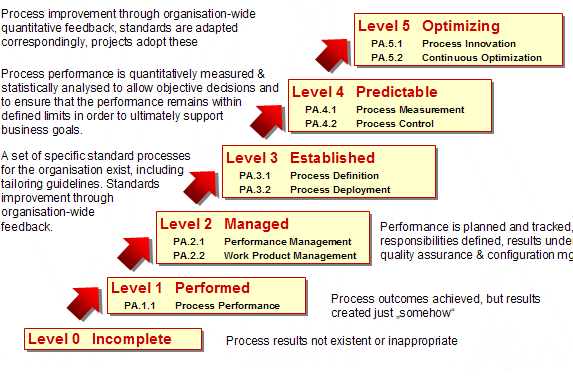
\includegraphics[scale=0.8]{./img/SPICE_capability_dimension.png}
\caption[Schema della capability dimension di SPICE]{Schema della \textit{capability dimension} di SPICE (tratta da SPiCE 1-2-1)}
\end{figure}
\newpage

\subsection{PDCA}
Il PDCA, conosciuto anche come \textit{Ciclo di Deming}, è un metodo di gestione dei processi durante il loro ciclo di vita con il fine di controllare il miglioramento continuo della loro qualità e, quindi, anche quella dei loro prodotti.
L'approccio che propone è suddiviso in quattro fasi da ripetere iterativamente fino al raggiungimento dell'obiettivo finale:
\begin{itemize}
\item \textbf{Plan}: fase di pianificazione in cui vengono stabiliti gli obiettivi ed i processi necessari per il raggiungimento dei risultati attesi;
\item \textbf{Do}: fase di esecuzione di quanto pianificato al punto precedente con rilevamento di dati significativi da poter analizzare nelle fasi successive;
\item \textbf{Check}: fase di controllo dei dati rilevati nella fase \textit{Do} per confrontare i risultati ottenuti con quelli attesi dalla fase \textit{Plan}. Le differenze riscontrate e le deviazioni nell'attuazione del piano osservate serviranno alla fase successiva;
\item \textbf{Act}: fase di attuazione del miglioramento della qualità, tramite l'adozione di strategie emerse dallo studio dei risultati della fase di \textit{Check}, eventualmente anche al di fuori del processo in questione.
\end{itemize}

\begin{figure}[httb]
\centering
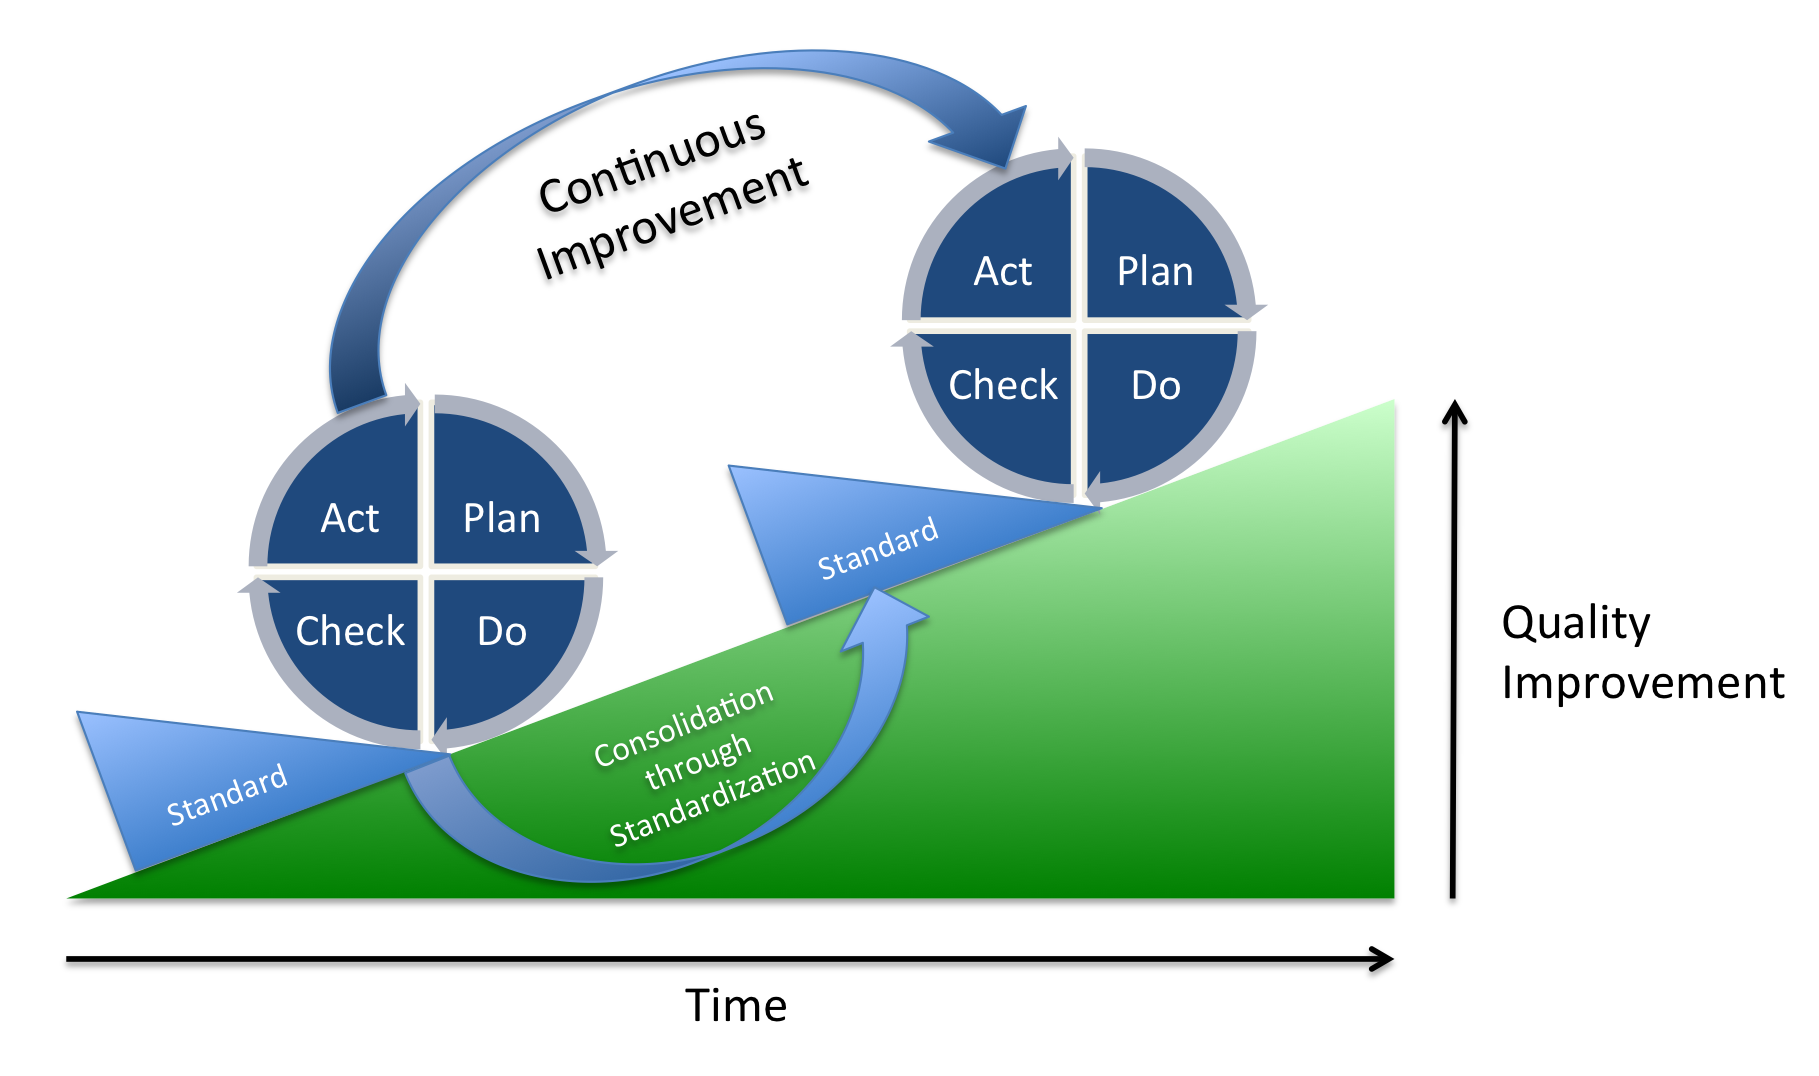
\includegraphics[scale=0.23]{./img/PDCA_applicazione.png}
\caption[Schema del miglioramento continuo tramite PDCA]{Schema del miglioramento continuo tramite PDCA (creato da Johannes Vietze)}
\end{figure}
\newpage

\subsection{ISO/IEC 9126}
Lo standard ISO/IEC 9126 fornisce un modello per la definizione della qualità di un software.

In particolare, esso distingue tre punti di vista sul software rispetto ai quali valutarne la qualità:
\begin{itemize}
\item \textbf{Qualità interna}: relativa al software sorgente non in esecuzione ed alla documentazione correlata. Viene rilevata tramite analisi statica ed è influenzata dalla qualità dei processi del ciclo di vita del prodotto;
\item \textbf{Qualità esterna}: relativa al software in esecuzione. Viene rilevata tramite test, in funzione degli obiettivi stabiliti, ed è influenzata dalla qualità interna;
\item \textbf{Qualità in uso}: relativa alla percezione dell'utente del prodotto finito in contesti reali d'uso. È influenzata dalla qualità esterna.
\end{itemize}

\begin{figure}[httb]
\centering
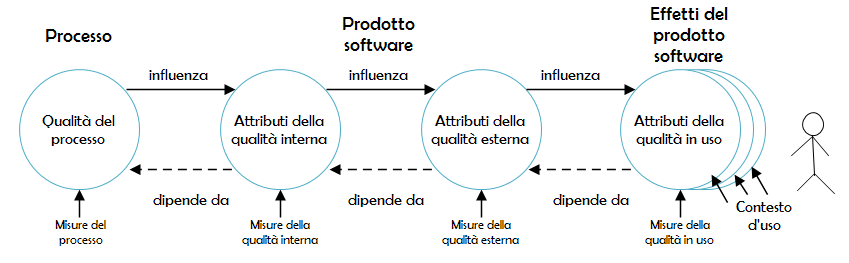
\includegraphics[scale=0.6]{./img/ciclo_di_qualita.png}
\caption[Schema del ciclo di qualità  del software]{Schema del ciclo di qualità del software (creato da Giuseppe Manuele)}
\end{figure}

Per ciascuno dei punti di vista vengono inoltre delineate delle caratteristiche e sotto-caratteristiche qualitative, eventualmente misurabili quantitativamente, mediante apposite metriche.

Per la qualità interna ed esterna esse sono:
\begin{itemize}
\item \textbf{Funzionabilità}: capacità di fornire funzioni che soddisfino le esigenze stabilite, nei relativi contesti di presentazione.
	\begin{itemize}
	\item \textbf{appropriatezza};
	\item \textbf{accuratezza};
	\item \textbf{interoperabilità};
	\item \textbf{conformità};
	\item \textbf{sicurezza}.
	\end{itemize}
\item \textbf{Affidabilità}: capacità di mantenere un determinato livello di prestazioni in date condizioni per un dato periodo.
	\begin{itemize}
	\item \textbf{maturità};
	\item \textbf{tolleranza agli errori};
	\item \textbf{recuperabilità};
	\item \textbf{aderenza}.
	\end{itemize}
\item \textbf{Efficienza}: capacità di fornire appropriate prestazioni relativamente alle risorse utilizzate.
	\begin{itemize}
	\item \textbf{comportamento rispetto al tempo};
	\item \textbf{utilizzo di risorse};
	\item \textbf{conformità}.
	\end{itemize}
\item \textbf{Usabilità}: capacità del prodotto software di essere capito, appreso e usato dall'utente, al verificarsi di determinate condizioni.
	\begin{itemize}
	\item \textbf{comprensibilità};
	\item \textbf{apprendibilità};
	\item \textbf{operabilità};
	\item \textbf{attrattiva};
	\item \textbf{conformità}.
	\end{itemize}
\item \textbf{Manutenibilità}: capacità del prodotto software di essere modificato, corretto o migliorato facilmente nel tempo.
	\begin{itemize}
	\item \textbf{analizzabilità};
	\item \textbf{modificabilità};
	\item \textbf{stabilità};
	\item \textbf{testabilità};
	\item \textbf{collaudabilità}.
	\end{itemize}
\item \textbf{Portabilità}: capacità del prodotto software di essere trasportato da un ambiente di lavoro all'altro.
	\begin{itemize}
	\item \textbf{adattabilità};
	\item \textbf{installabilità};
	\item \textbf{conformità};
	\item \textbf{sostituibilità}.
	\end{itemize}
\end{itemize}

Le caratteristiche per la qualità in uso sono:
\begin{itemize}
\item \textbf{Efficacia}: capacità di permettere all'utente di raggiungere gli obiettivi specificati con accuratezza e completezza;
\item \textbf{Produttività}: capacità di permettere all'utente di spendere una quantità di risorse appropriata all'efficacia ottenuta dall'uso del prodotto;
\item \textbf{Soddisfacibilità}: capacità di soddisfare l'utente;
\item \textbf{Sicurezza}: capacità di raggiungere accettabili livelli di rischio nei confronti di persone e dell'ambiente di lavoro.
\end{itemize}

\begin{figure}[httb]
\centering
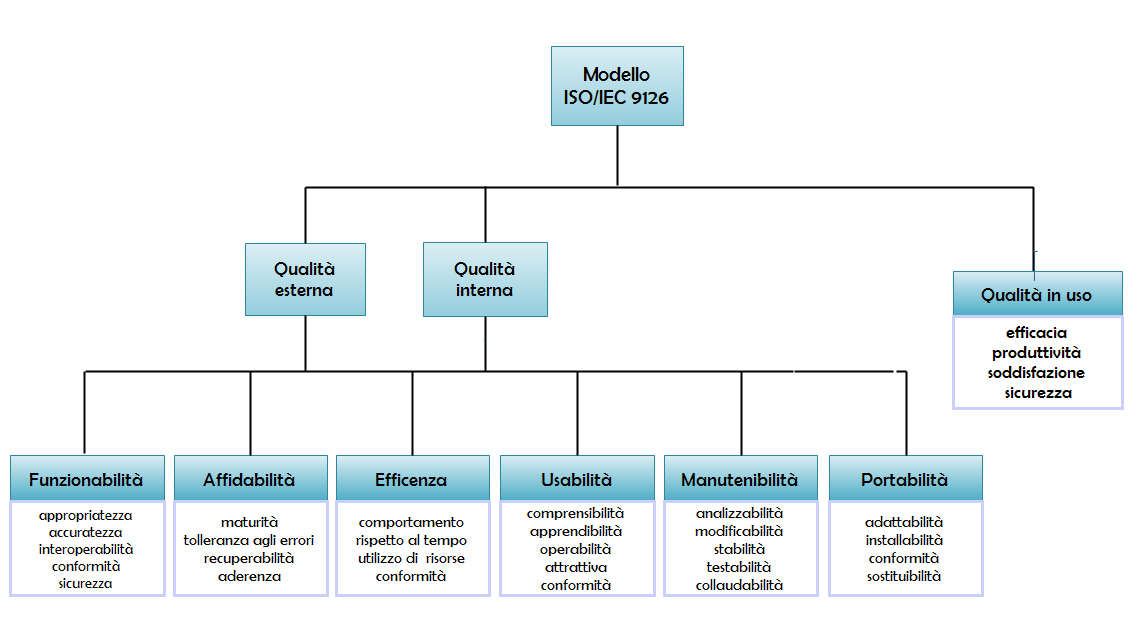
\includegraphics[scale=0.5]{./img/ISO-IEC_9126_schema.png}
\caption[Schema delle caratteristiche definite in ISO/IEC 9126]{Schema delle caratteristiche definite in ISO/IEC 9126 (creato da Giuseppe Manuele)}
\end{figure}